\documentclass[12pt,a4paper]{article}

\usepackage[utf8]{inputenc}
\usepackage[T1]{fontenc}
\usepackage[polish]{babel}
\usepackage{lmodern}
\usepackage{amsmath}
\usepackage{amssymb}
\usepackage{booktabs}
\usepackage{graphicx}
\usepackage{float}
\usepackage{geometry}
\usepackage{hyperref}
\usepackage{setspace}
\usepackage{array}

\geometry{margin=2.5cm}
\onehalfspacing
\graphicspath{{../figures/}}

\title{Bayesowska analiza determinant wysokiego dochodu\\
\large Praca domowa 2 z ekonometrii bayesowskiej}
\author{Jakub Mikołajczak, 121732}
\date{10 czerwca 2026}

\begin{document}
\maketitle

\section{Cel i odniesienie do pierwszej pracy domowej}

Celem pracy jest kontynuacja analizy przeprowadzonej w pierwszej pracy domowej,
w której badano determinanty uzyskiwania dochodu powyżej 50 tys. dolarów rocznie
na podstawie zbioru Adult Census Income. W pierwszej pracy zastosowano
bayesowski liniowy model prawdopodobieństwa z rozkładem normalnym-gamma i
rozwiązaniem analitycznym. Takie podejście było wygodne rachunkowo, lecz ma
ograniczenie merytoryczne: dla zmiennej binarnej liniowy model
prawdopodobieństwa może generować wartości oczekiwane spoza przedziału
$[0,1]$.

W tej pracy model zostaje zmieniony na bayesowski model logitowy. Jest to
naturalne rozszerzenie poprzedniej analizy, ponieważ zmienna objaśniana
\texttt{income\_high} przyjmuje wartość 1 dla osób z dochodem powyżej 50 tys.
dolarów rocznie oraz 0 w przeciwnym przypadku. Zamiast rozwiązania
analitycznego zastosowano estymację numeryczną w pakiecie \texttt{rstan}. W
praktyce wykorzystano algorytm NUTS (No-U-Turn Sampler), czyli adaptacyjną
odmianę metody HMC, standardowo stosowaną w Stan do próbkowania z rozkładów a
posteriori. Pozwala to wykorzystać techniki omawiane na zajęciach dotyczące
MCMC, diagnostyki zbieżności oraz predykcji bayesowskiej.

\section{Dane i przygotowanie próby}

Wykorzystano ten sam zbiór danych co w pierwszej pracy: Adult Census Income,
pochodzący z bazy Census Bureau i opisany w pliku \texttt{adult.names}. Analizę
ograniczono do obserwacji dotyczących Stanów Zjednoczonych, a następnie
wylosowano próbę 500 obserwacji. Ziarno losowania próby zapisano w kodzie jako
\texttt{DATA\_SEED = 121732}.

\begin{table}[H]
\centering
\caption{Podstawowe informacje o próbie}
\small
\begin{tabular}{lr}
\toprule
Informacja & Wartość \\
\midrule
Obserwacje w pliku \texttt{adult.data} & 32\,561 \\
Obserwacje z USA & 29\,170 \\
Wylosowana próba & 500 \\
Udział \texttt{income\_high = 1} w próbie & 0{,}258 \\
\bottomrule
\end{tabular}
\end{table}

Zmienna objaśniana ma postać:
\[
 y_i =
 \begin{cases}
 1, & \text{gdy dochód osoby } i \text{ przekracza 50 tys. dolarów rocznie},\\
 0, & \text{w przeciwnym przypadku.}
 \end{cases}
\]

W modelu wykorzystano te same predyktory co w pierwszej pracy domowej: poziom
edukacji, wiek, kwadrat standaryzowanego wieku, liczbę godzin pracy, płeć,
status małżeński oraz informację o dodatnich zyskach kapitałowych. Zmienne
ilościowe zostały wystandaryzowane, dlatego ich parametry można interpretować
jako efekt wzrostu zmiennej o jedno odchylenie standardowe.

\section{Specyfikacja modelu}

Dla obserwacji $i=1,\ldots,n$ przyjęto model:
\[
 y_i \sim \mathrm{Bernoulli}(p_i),
\]
\[
 \mathrm{logit}(p_i)
 =
 \log\left(\frac{p_i}{1-p_i}\right)
 =
 x_i^\top \beta.
\]

Wektor $x_i$ zawiera wyraz wolny oraz następujące zmienne:
\[
\begin{aligned}
 x_i = (&1,\ \mathrm{education\_z}_i,\ \mathrm{age\_z}_i,\ \mathrm{age\_z2}_i,\\
       &\mathrm{hours\_z}_i,\ \mathrm{sex\_male}_i,\ \mathrm{married}_i,
       \ \mathrm{capital\_gain\_ind}_i).
\end{aligned}
\]

Sukcesem w modelu jest zdarzenie \(\texttt{income\_high}=1\). Szansa tego
zdarzenia jest równa \(p_i/(1-p_i)\). Współczynnik \(\beta_j\) opisuje zmianę
logarytmu szans, czyli zmianę wartości \(\log(p_i/(1-p_i))\), przy wzroście
danej zmiennej o jednostkę, przy pozostałych zmiennych ustalonych. Po
przekształceniu wykładniczym \(\exp(\beta_j)\) otrzymujemy iloraz szans, czyli
odds ratio (OR). Iloraz szans porównuje dwie szanse: po zmianie danej cechy i
przed jej zmianą. Dzięki temu model logitowy daje interpretację naturalną dla
zmiennej zero-jedynkowej i utrzymuje prognozowane prawdopodobieństwa w
przedziale $[0,1]$.

\section{Elicytacja rozkładów a priori}

Zgodnie z poleceniem pracy zastosowano rozkład a priori inny niż normalny-gamma.
Dla każdego parametru regresji przyjęto rozkład t-Studenta:
\[
 \beta_j \sim t_{\nu}(m_j, s_j),
\]
gdzie \(\nu=4\) oznacza liczbę stopni swobody, \(m_j\) to wartość centralna
prioru, a \(s_j\) to jego skala. W kodzie odpowiadają im odpowiednio obiekty
z wartościami położenia i skali prioru. Rozkład t-Studenta ma grubsze ogony niż
rozkład normalny, więc dopuszcza większe odchylenia od wartości centralnej niż
analogiczny prior normalny.

Przyjęte priory są umiarkowanie informacyjne. Są wynikiem subiektywnej, ekonomicznie
uzasadnionej elicytacji, opartej na teorii kapitału ludzkiego, intuicji
ekonomicznej oraz kierunkach efektów otrzymanych w pierwszej pracy domowej.

Elicytację przeprowadzono na skali ilorazów szans. Jeżeli przed obserwacją
próby oczekiwano, że dana cecha zmienia szanse wysokiego dochodu \(OR_j\) razy,
to środek prioru dla współczynnika logitowego ustawiono jako:
\[
 m_j = \log(OR_j).
\]
Dla wyrazu wolnego nie ma ilorazu szans związanego ze zmianą predyktora. Dlatego
przyjęto bazowe prawdopodobieństwo wysokiego dochodu \(p_0=0{,}25\) i
przekształcono je przez logit:
\[
 m_0 = \log\left(\frac{p_0}{1-p_0}\right) = \mathrm{logit}(0{,}25)=-1{,}099.
\]

\begin{table}[H]
\centering
\caption{Położenie priorów po przekształceniu na skalę log-szans}
\small
\begin{tabular}{lrr}
\toprule
Parametr & Założenie na skali OR / \(p_0\) & Położenie prioru \(m_j\) \\
\midrule
\texttt{(Intercept)} & \(p_0=0{,}25\) & -1{,}099 \\
\texttt{education\_z} & 1{,}60 & 0{,}470 \\
\texttt{age\_z} & 1{,}30 & 0{,}262 \\
\texttt{age\_z2} & 0{,}85 & -0{,}163 \\
\texttt{hours\_z} & 1{,}25 & 0{,}223 \\
\texttt{sex\_male} & 1{,}40 & 0{,}336 \\
\texttt{married} & 2{,}00 & 0{,}693 \\
\texttt{capital\_gain\_ind} & 3{,}00 & 1{,}099 \\
\bottomrule
\end{tabular}
\end{table}

Tabela pokazuje tę samą elicytację po przeniesieniu na skalę współczynników
modelu logitowego.

\begin{table}[H]
\centering
\caption{Uzasadnienie centralnych wartości priorów na skali ilorazów szans}
\scriptsize
\begin{tabular}{lrl}
\toprule
Zmienna & Centralne OR & Uzasadnienie \\
\midrule
\texttt{education\_z} & 1{,}60 & Edukacja jest podstawową zmienną teorii kapitału ludzkiego. \\
\texttt{age\_z} & 1{,}30 & Wiek przybliża doświadczenie i pozycję w cyklu życia. \\
\texttt{age\_z2} & 0{,}85 & Dodatni wpływ wieku powinien słabnąć wraz z wiekiem. \\
\texttt{hours\_z} & 1{,}25 & Liczba godzin pracy powinna umiarkowanie zwiększać szanse dochodu. \\
\texttt{sex\_male} & 1{,}40 & Możliwy dodatni efekt płci męskiej, ale z dużą niepewnością. \\
\texttt{married} & 2{,}00 & Stan małżeński może sygnalizować stabilność ekonomiczną. \\
\texttt{capital\_gain\_ind} & 3{,}00 & Dodatnie zyski kapitałowe są silnym sygnałem zamożności. \\
\bottomrule
\end{tabular}
\end{table}

Wartości OR są założeniami przed analizą, dobranymi tak, aby kierunki efektów były zgodne z interpretacją
ekonomiczną i wynikami pierwszej pracy. Skala prioru określa szerokość rozkładu
na skali logarytmu szans. Większa skala oznacza większą niepewność co do efektu.
Największą skalę przyjęto dla \texttt{capital\_gain\_ind}, ponieważ efekt
dodatnich zysków kapitałowych może być silny i zmienny. Zmienne zero-jedynkowe
\texttt{sex\_male} i \texttt{married} mają większą skalę niż większość zmiennych
ilościowych, bo ich efekty mogą być bardziej heterogeniczne. Mniejsze skale dla
\texttt{age\_z2} i \texttt{hours\_z} odzwierciedlają oczekiwanie raczej
umiarkowanych efektów. Wyraz wolny ma dużą skalę, ponieważ bazowe
prawdopodobieństwo wysokiego dochodu jest niepewne po ograniczeniu próby.

Przyjęto \(\nu=4\), ponieważ rozkład t-Studenta z taką liczbą stopni swobody ma
wyraźnie grubsze ogony niż rozkład normalny, ale nadal zachowuje skończoną
wariancję. Jest to kompromis między priorami zbyt restrykcyjnymi a priorami
zbyt rozproszonymi.

\section{Estymacja MCMC w Stan}

Model oszacowano w pakiecie \texttt{rstan}. Użyto 4 łańcuchów, 4000 iteracji na
łańcuch, w tym 1000 iteracji rozgrzewki (warm-up). Ziarno próbkowania MCMC
wynosi 20260609. Ustawienia algorytmu to \texttt{adapt\_delta} równe 0{,}95
oraz \texttt{max\_treedepth} równe 12.

W trakcie próbkowania algorytm nie zgłaszał problematycznych przejść przez
przestrzeń parametrów (tzw. divergent transitions) ani przekroczeń maksymalnej
głębokości drzewa. Oznacza to, że algorytm nie sygnalizował istotnych problemów
numerycznych w eksploracji rozkładu a posteriori.

\begin{table}[H]
\centering
\caption{Efektywna liczba próbek w diagnostyce MCMC}
\small
\begin{tabular}{lr}
\toprule
Parametr & Efektywna liczba próbek \\
\midrule
\texttt{(Intercept)} & 7\,662 \\
\texttt{education\_z} & 11\,357 \\
\texttt{age\_z} & 9\,234 \\
\texttt{age\_z2} & 8\,458 \\
\texttt{hours\_z} & 13\,155 \\
\texttt{sex\_male} & 9\,130 \\
\texttt{married} & 8\,305 \\
\texttt{capital\_gain\_ind} & 12\,308 \\
\bottomrule
\end{tabular}
\end{table}

Dla wszystkich parametrów \(\hat{R}\) wynosi około 1. Wartość \(\hat{R}\)
porównuje zmienność między łańcuchami ze zmiennością wewnątrz łańcuchów;
wartości bliskie 1 wskazują, że łańcuchy dają zgodne wyniki. Wysokie wartości
efektywnej liczby próbek oznaczają, że mimo autokorelacji losowań MCMC uzyskano
dużą ilość użytecznej informacji o rozkładzie a posteriori.

\begin{figure}[H]
\centering
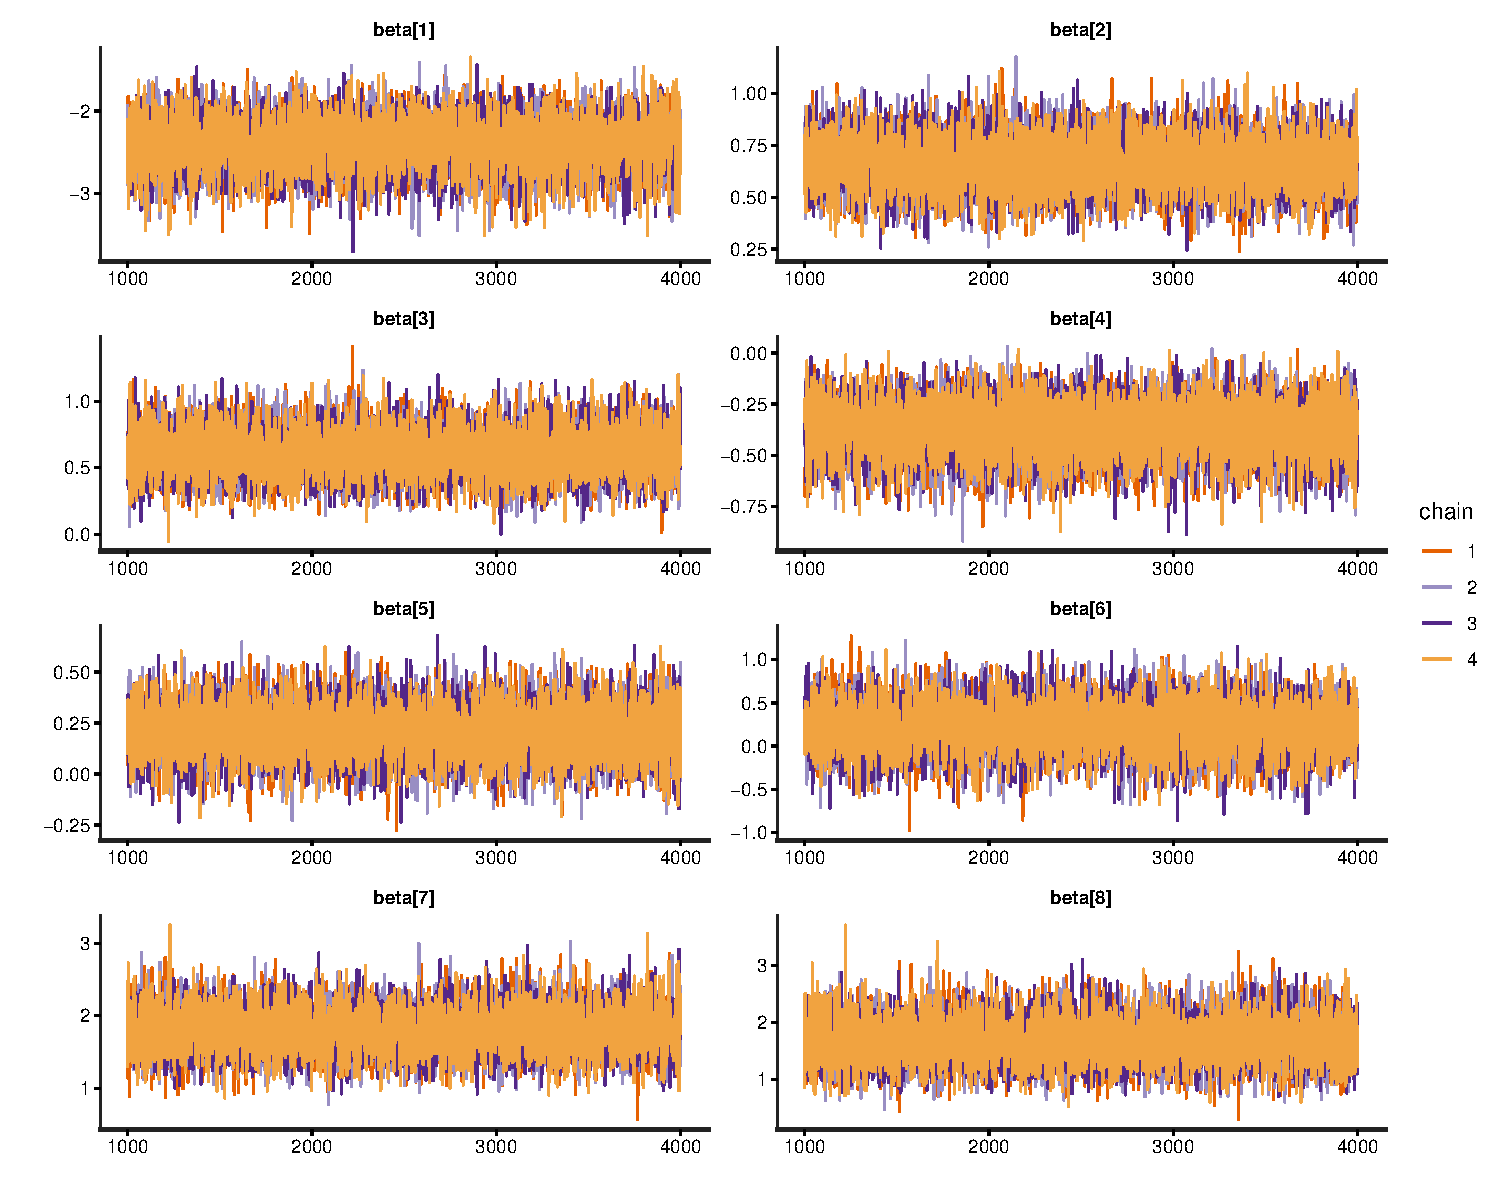
\includegraphics[width=\textwidth]{traceplot_beta.pdf}
\caption{Przebieg łańcuchów MCMC dla parametrów modelu logitowego}
\end{figure}

Wykresy przebiegu łańcuchów nie pokazują wyraźnych trendów, dryfu ani
rozdzielenia między łańcuchami. Poszczególne łańcuchy nakładają się na siebie i
oscylują wokół podobnych poziomów, co jest zgodne z wnioskiem o poprawnym
mieszaniu łańcuchów. Ocena wizualna jest spójna z wartościami \(\hat{R}\)
bliskimi 1.

\section{Rozkłady a posteriori}

Tabela poniżej przedstawia średnie a posteriori, odchylenia standardowe,
95-procentowe przedziały HPDI, prawdopodobieństwo \(P(\beta_j>0\mid y)\) oraz
przybliżony czynnik Bayesa \(BF_{10}\) dla hipotezy alternatywnej
\(\beta_j \neq 0\) względem hipotezy punktowej \(\beta_j=0\).

\begin{table}[H]
\centering
\caption{Podsumowanie rozkładów a posteriori parametrów modelu}
\scriptsize
\resizebox{\textwidth}{!}{
\begin{tabular}{llrrrrrr}
\toprule
Parametr & Opis & Średnia & SD & HPDI dolny & HPDI górny & \(P(\beta>0\mid y)\) & BF10 \\
\midrule
\texttt{(Intercept)} & wyraz wolny & -2{,}408 & 0{,}306 & -3{,}009 & -1{,}818 & 0{,}000 & 25495{,}98 \\
\texttt{education\_z} & edukacja, +1 SD & 0{,}658 & 0{,}122 & 0{,}424 & 0{,}898 & 1{,}000 & 16927{,}56 \\
\texttt{age\_z} & wiek, +1 SD & 0{,}615 & 0{,}169 & 0{,}300 & 0{,}968 & 1{,}000 & 295{,}89 \\
\texttt{age\_z2} & kwadrat wieku & -0{,}374 & 0{,}127 & -0{,}622 & -0{,}124 & 0{,}001 & 37{,}59 \\
\texttt{hours\_z} & godziny pracy, +1 SD & 0{,}209 & 0{,}124 & -0{,}037 & 0{,}451 & 0{,}953 & 1{,}17 \\
\texttt{sex\_male} & mężczyzna & 0{,}215 & 0{,}278 & -0{,}334 & 0{,}757 & 0{,}789 & 0{,}58 \\
\texttt{married} & w małżeństwie & 1{,}796 & 0{,}306 & 1{,}226 & 2{,}402 & 1{,}000 & 35548{,}36 \\
\texttt{capital\_gain\_ind} & dodatnie zyski kapitałowe & 1{,}684 & 0{,}386 & 0{,}942 & 2{,}441 & 1{,}000 & 27768{,}55 \\
\bottomrule
\end{tabular}}
\end{table}

Najsilniejsze efekty dodatnie dotyczą stanu małżeńskiego, dodatnich zysków
kapitałowych, edukacji oraz wieku. W każdym z tych przypadków przedziały HPDI
leżą powyżej zera, a
\(P(\beta>0\mid y)\) jest praktycznie równe 1. Ujemny efekt
\texttt{age\_z2} odpowiada wygasaniu dodatniego wpływu wieku. Zmienna
\texttt{hours\_z} ma dodatni efekt średni, ale dowód jest słabszy, ponieważ HPDI
obejmuje okolice zera. Dla \texttt{sex\_male} również nie ma jednoznacznego
wsparcia: HPDI obejmuje zero, a \(BF_{10}\) jest mniejszy niż 1.

\begin{figure}[H]
\centering
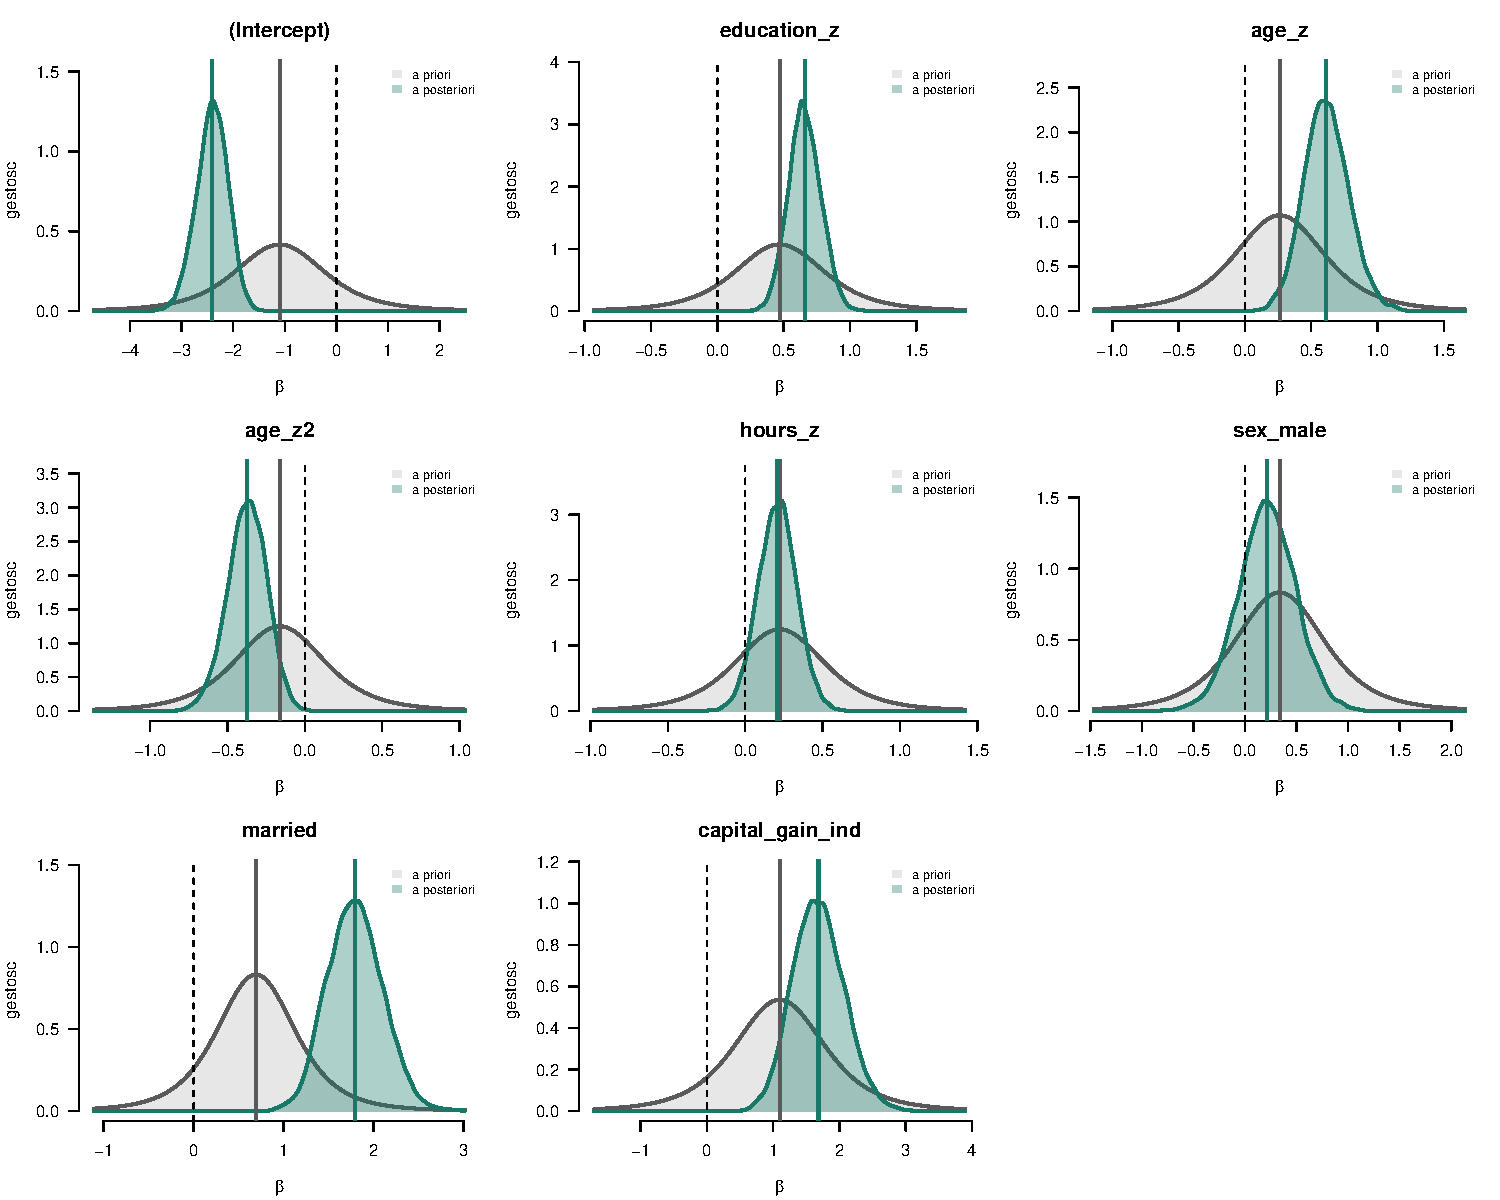
\includegraphics[width=\textwidth]{prior_vs_posterior_beta.pdf}
\caption{Porównanie rozkładów a priori i a posteriori dla parametrów \(\beta\)}
\end{figure}

\begin{figure}[H]
\centering
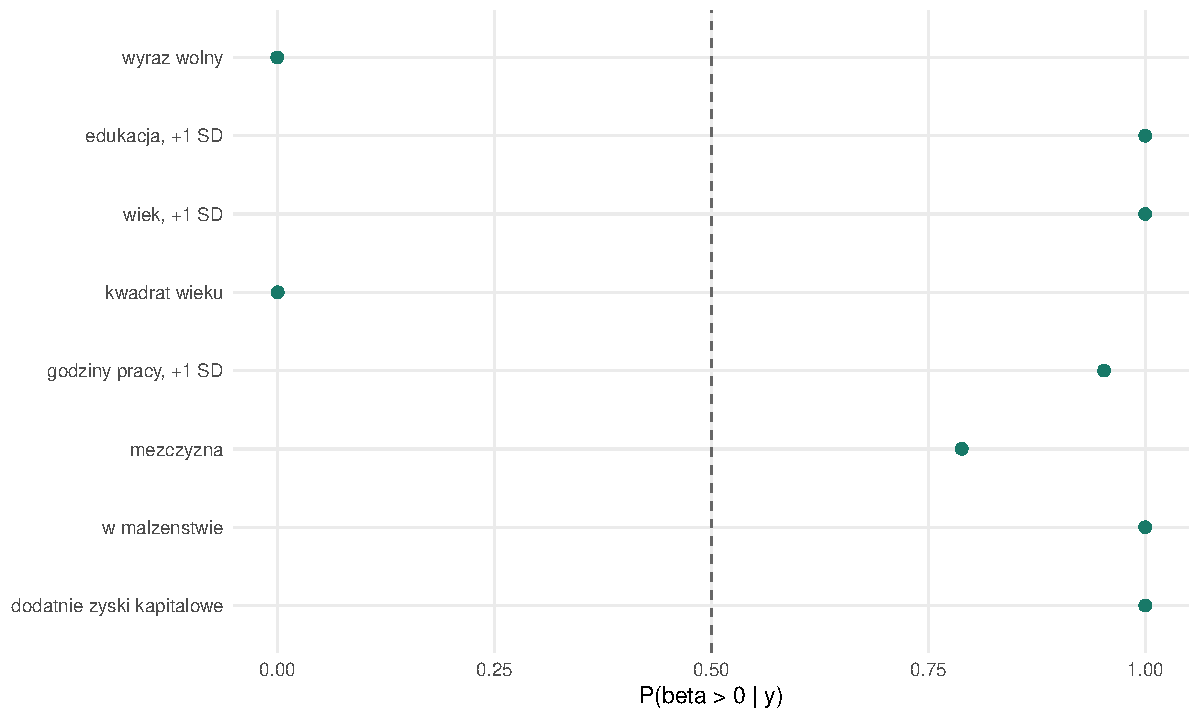
\includegraphics[width=0.85\textwidth]{posterior_probability_positive.pdf}
\caption{Prawdopodobieństwa a posteriori dodatniego wpływu zmiennych}
\end{figure}

\section{Interpretacja przez ilorazy szans}

Ponieważ parametry modelu logitowego są mierzone na skali logarytmu szans,
wyniki warto interpretować również przez \(\exp(\beta_j)\).

\begin{table}[H]
\centering
\caption{Ilorazy szans wynikające z rozkładów a posteriori}
\scriptsize
\resizebox{\textwidth}{!}{
\begin{tabular}{llrrrr}
\toprule
Parametr & Opis & Średnia OR & Mediana OR & HPDI dolny & HPDI górny \\
\midrule
\texttt{education\_z} & edukacja, +1 SD & 1{,}946 & 1{,}924 & 1{,}489 & 2{,}410 \\
\texttt{age\_z} & wiek, +1 SD & 1{,}876 & 1{,}840 & 1{,}291 & 2{,}537 \\
\texttt{age\_z2} & kwadrat wieku & 0{,}694 & 0{,}691 & 0{,}522 & 0{,}865 \\
\texttt{hours\_z} & godziny pracy, +1 SD & 1{,}242 & 1{,}234 & 0{,}956 & 1{,}559 \\
\texttt{sex\_male} & mężczyzna & 1{,}289 & 1{,}241 & 0{,}674 & 2{,}057 \\
\texttt{married} & w małżeństwie & 6{,}322 & 5{,}988 & 3{,}064 & 10{,}388 \\
\texttt{capital\_gain\_ind} & dodatnie zyski kapitałowe & 5{,}815 & 5{,}323 & 2{,}103 & 10{,}448 \\
\bottomrule
\end{tabular}}
\end{table}

Mediana ilorazu szans dla \texttt{married} wynosi 5{,}988, co oznacza, że przy
pozostałych cechach ustalonych osoby pozostające w małżeństwie mają znacznie
wyższe szanse dochodu powyżej 50 tys. dolarów. Dla dodatnich zysków kapitałowych
mediana ilorazu szans wynosi 5{,}323. Wzrost edukacji o jedno odchylenie
standardowe odpowiada medianie ilorazu szans 1{,}924, a wzrost wieku o jedno
odchylenie standardowe medianie 1{,}840. Współczynnik przy kwadracie wieku daje
iloraz szans poniżej 1, co potwierdza wygasanie dodatniego efektu wieku.

\begin{figure}[H]
\centering
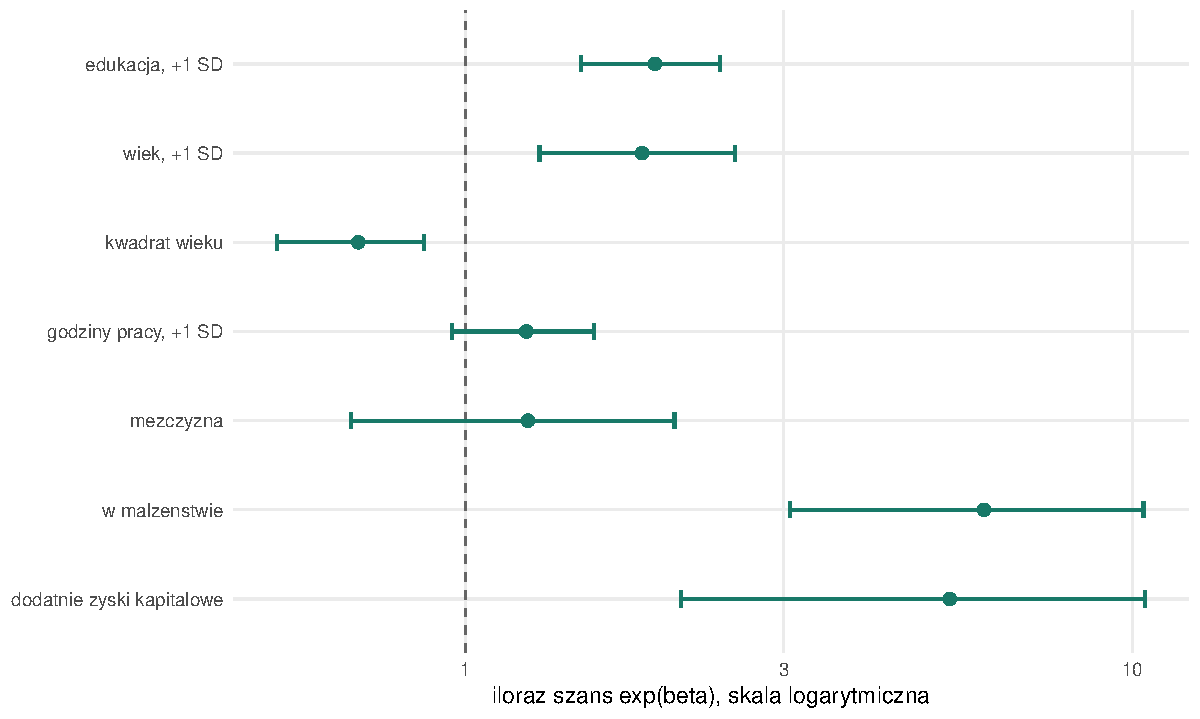
\includegraphics[width=0.85\textwidth]{odds_ratios_hpdi.pdf}
\caption{Ilorazy szans i 95-procentowe przedziały HPDI}
\end{figure}

\section{Predykcja bayesowska}

Prognozę wykonano dla pierwszej obserwacji z wylosowanej próby, tak aby
predykcja była w pełni replikowalna. Dla każdej próbki MCMC obliczono
prawdopodobieństwo \(p_{\mathrm{new}}\), a następnie wygenerowano predykcję
posterior predictive:
\[
 y_{\mathrm{new}}^{rep} \sim
 \mathrm{Bernoulli}(p_{\mathrm{new}}).
\]

\begin{table}[H]
\centering
\caption{Predykcja bayesowska dla pierwszej obserwacji z próby}
\small
\begin{tabular}{lr}
\toprule
Wielkość & Wartość \\
\midrule
Numer obserwacji & 1 \\
Obserwowana klasa & 0 \\
Średnie prawdopodobieństwo a posteriori & 0{,}253 \\
Mediana prawdopodobieństwa a posteriori & 0{,}250 \\
Dolna granica 95\% HPDI & 0{,}157 \\
Górna granica 95\% HPDI & 0{,}361 \\
Predykcyjne prawdopodobieństwo klasy 1 & 0{,}254 \\
\bottomrule
\end{tabular}
\end{table}

\begin{figure}[H]
\centering
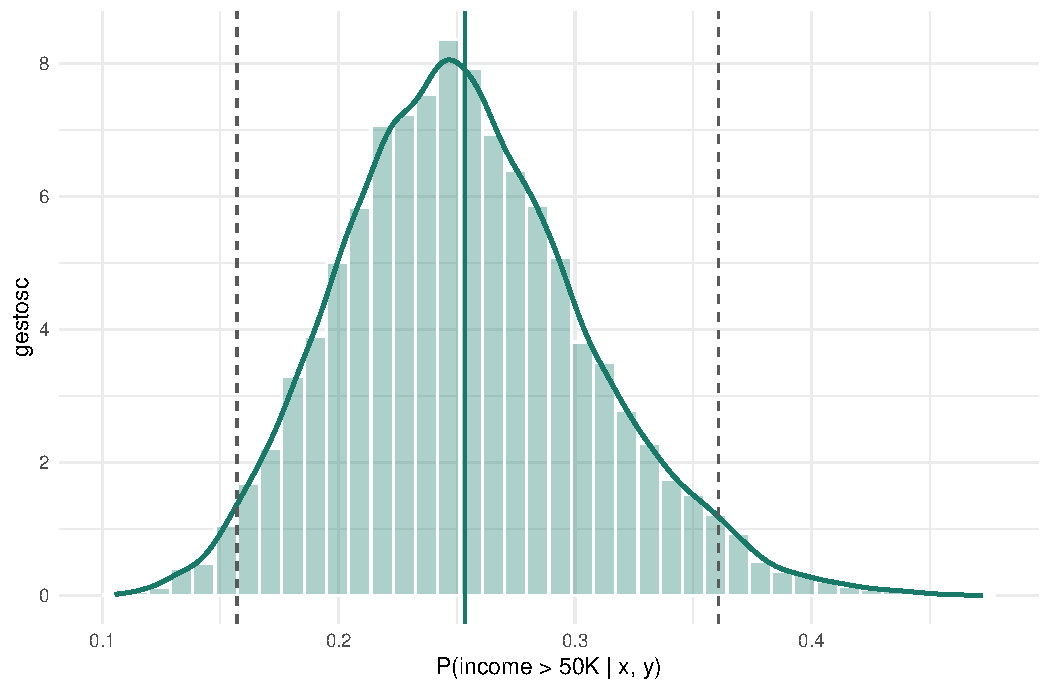
\includegraphics[width=0.75\textwidth]{prediction_probability_selected_observation.pdf}
\caption{Rozkład a posteriori prognozowanego prawdopodobieństwa dla wybranej obserwacji}
\end{figure}

Rysunek przedstawia niepewność dotyczącą prognozowanego prawdopodobieństwa
wysokiego dochodu dla wybranej obserwacji. Rozkład koncentruje się w okolicy
0{,}25, a 95-procentowy przedział HPDI mieści się mniej więcej między 0{,}16 a
0{,}36. Ponieważ obserwowana klasa tej osoby wynosi 0, model przypisuje jej
raczej niskie prawdopodobieństwo przynależności do grupy wysokich dochodów, co
jest zgodne z obserwacją.

\begin{figure}[H]
\centering
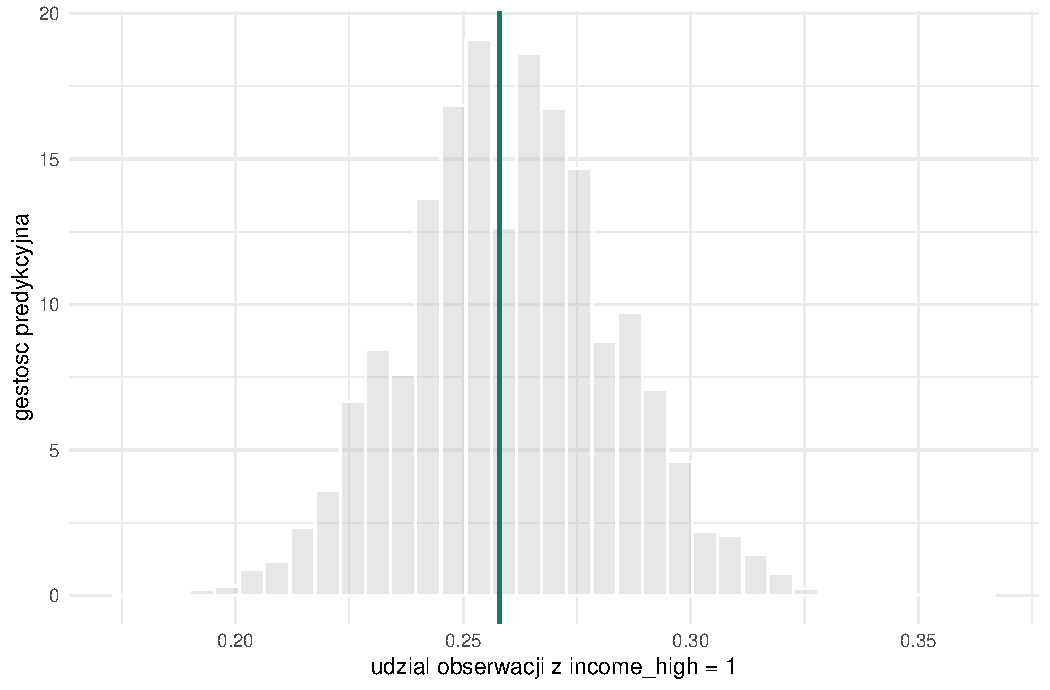
\includegraphics[width=0.75\textwidth]{posterior_predictive_check_income_rate.pdf}
\caption{Posterior predictive check dla udziału obserwacji z \texttt{income\_high}=1}
\end{figure}

Na tym wykresie każda wartość histogramu oznacza udział osób z
\texttt{income\_high = 1} w jednej sztucznie wygenerowanej próbie z rozkładu
predykcyjnego modelu. Innymi słowy, dla każdego losowania z posteriora model
symuluje, ile osób w próbie miałoby dochód powyżej 50 tys. dolarów, a następnie
liczony jest udział takich osób. Pionowa zielona linia pokazuje rzeczywisty
udział klasy 1 w danych. Jeżeli linia znajduje się w typowym obszarze
histogramu, to model dobrze odtwarza przynajmniej ogólną częstość wysokich
dochodów w próbie. Ten wykres nie ocenia jeszcze, czy model poprawnie klasyfikuje
każdą osobę, ale sprawdza, czy generowane przez niego dane mają realistyczny
łączny udział obserwacji z wysokim dochodem.

\section{Porównanie z podejściem z pierwszej pracy}

Wyniki drugiej pracy są zasadniczo zgodne z kierunkami efektów uzyskanymi w
pierwszej pracy. Edukacja ma dodatni wpływ na prawdopodobieństwo wysokiego
dochodu, wiek działa dodatnio, a kwadrat wieku ujemnie, co odpowiada efektowi
wygasania korzyści z wieku lub doświadczenia. Liczba godzin pracy ma dodatni,
ale słabszy efekt. Stan małżeński i dodatnie zyski kapitałowe pozostają
najsilniejszymi dodatnimi predyktorami. Efekt płci męskiej jest dodatni w
średniej, ale w modelu logitowym nie ma jednoznacznego wsparcia posteriorowego,
ponieważ przedział HPDI obejmuje zero.

Wartości parametrów z obu modeli nie są bezpośrednio porównywalne, ponieważ w
liniowym modelu prawdopodobieństwa współczynniki wyrażają zmianę
prawdopodobieństwa w punktach procentowych, natomiast w modelu logitowym opisują
zmianę logarytmu szans. Porównywalne są przede wszystkim kierunki efektów,
względna siła zmiennych oraz jakość predykcyjna.

Drugie podejście jest teoretycznie lepiej dopasowane do binarnej zmiennej
zależnej, ponieważ respektuje zakres prawdopodobieństw i pozwala interpretować
wyniki przez ilorazy szans. Nie oznacza to automatycznie radykalnie innych
wniosków empirycznych. W tej próbie główne wnioski są podobne do pierwszej
pracy, ale model logitowy daje bardziej właściwą strukturę probabilistyczną i
bardziej naturalną interpretację dla danych binarnych. W praktyce druga praca
nie obala wyników pierwszej, lecz przedstawia je w modelu lepiej dostosowanym do
zmiennej zero-jedynkowej.

\end{document}
